% Vietnamese translation for OI Public Library
% Source-PDF: IOI中国国家候选队论文/2002/黄芸.pdf
\documentclass[11pt]{article}
\usepackage{oipl-vn}
\usepackage{tikz}

\title{POI0110 Dancing Flies: đẳng cấu đồ thị}
\author{Huang Yun}
\date{}

\begin{document}
\maketitle

\origtitle{POI0110 Dancing Flies}
\sourcepath{IOI China candidate team papers / 2002 / Huang Yun.pdf}

\tableofcontents

\section{Đề bài}

Có một loài ruồi nhảy múa rất kỳ lạ. Khi chúng biểu diễn, trước hết người ta
đặt trên bàn \(n\) đồng xu, đánh số từ \(1\) đến \(n\). Bên cạnh mỗi đồng xu có
một dòng ghi chú dạng \(i\to j\): \(i\) là số hiệu của đồng xu này, còn \(j\)
là số hiệu của đồng xu mà con ruồi đang đứng trên đồng xu \(i\) phải bay đến ở
bước tiếp theo. Người ta đặt một con ruồi lên mỗi đồng xu, rồi các con ruồi bắt
đầu nhảy múa theo các dòng ghi chú đó.

Vì vậy, các dòng ghi chú trên đồng xu xác định toàn bộ màn biểu diễn. Tuy
nhiên, hai cách đặt ghi chú khác nhau vẫn có thể tạo ra cùng một màn biểu diễn,
miễn là ta được đổi cách tương ứng các đồng xu.

\begin{center}
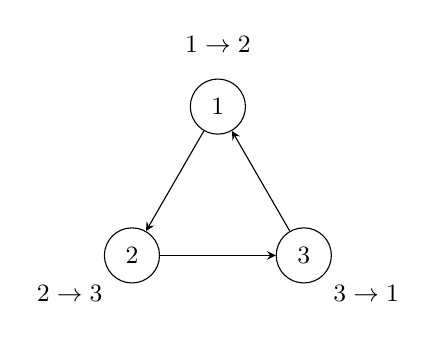
\begin{tikzpicture}[>=stealth,scale=0.9,every node/.style={font=\small}]
  \node[circle,draw,minimum size=7mm] (a) at (90:1.4) {1};
  \node[circle,draw,minimum size=7mm] (b) at (210:1.4) {2};
  \node[circle,draw,minimum size=7mm] (c) at (330:1.4) {3};
  \draw[->] (a) -- (b);
  \draw[->] (b) -- (c);
  \draw[->] (c) -- (a);
  \node at (a.north) [above=2mm] {\(1\to2\)};
  \node at (b.south west) [below left=0mm] {\(2\to3\)};
  \node at (c.south east) [below right=0mm] {\(3\to1\)};
\end{tikzpicture}
\end{center}

\subsection{Ví dụ 1}

\[
\begin{array}{c@{\qquad\qquad}c}
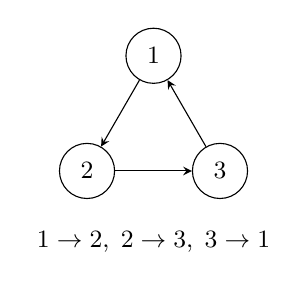
\begin{tikzpicture}[>=stealth,scale=0.75,every node/.style={font=\small}]
  \node[circle,draw,minimum size=7mm] (a) at (90:1.3) {1};
  \node[circle,draw,minimum size=7mm] (b) at (210:1.3) {2};
  \node[circle,draw,minimum size=7mm] (c) at (330:1.3) {3};
  \draw[->] (a) -- (b);
  \draw[->] (b) -- (c);
  \draw[->] (c) -- (a);
  \node at (0,-1.85) {\(1\to2,\;2\to3,\;3\to1\)};
\end{tikzpicture}
&
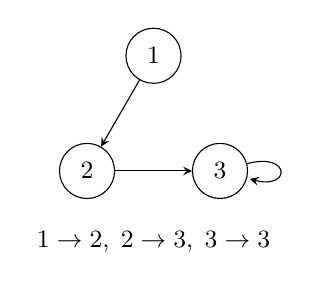
\begin{tikzpicture}[>=stealth,scale=0.75,every node/.style={font=\small}]
  \node[circle,draw,minimum size=7mm] (a) at (90:1.3) {1};
  \node[circle,draw,minimum size=7mm] (b) at (210:1.3) {2};
  \node[circle,draw,minimum size=7mm] (c) at (330:1.3) {3};
  \draw[->] (a) -- (b);
  \draw[->] (b) -- (c);
  \draw[->] (c) edge[loop right] (c);
  \node at (0,-1.85) {\(1\to2,\;2\to3,\;3\to3\)};
\end{tikzpicture}
\end{array}
\]

Hai màn biểu diễn này khác nhau: bên trái là một vòng có ba đồng xu, còn bên
phải là một dây đi vào một vòng tự khép tại đồng xu \(3\).

\subsection{Ví dụ 2}

\[
\begin{array}{c@{\qquad\qquad}c}
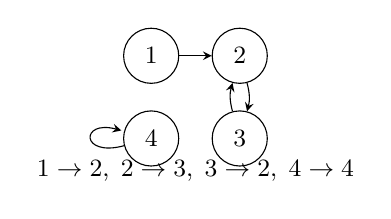
\begin{tikzpicture}[>=stealth,scale=0.75,every node/.style={font=\small}]
  \node[circle,draw,minimum size=7mm] (a) at (0,1.4) {1};
  \node[circle,draw,minimum size=7mm] (b) at (1.5,1.4) {2};
  \node[circle,draw,minimum size=7mm] (c) at (1.5,0) {3};
  \node[circle,draw,minimum size=7mm] (d) at (0,0) {4};
  \draw[->] (a) -- (b);
  \draw[->] (b) to[bend left=15] (c);
  \draw[->] (c) to[bend left=15] (b);
  \draw[->] (d) edge[loop left] (d);
  \node at (0.75,-0.55) {\(1\to2,\;2\to3,\;3\to2,\;4\to4\)};
\end{tikzpicture}
&
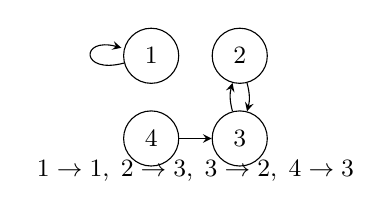
\begin{tikzpicture}[>=stealth,scale=0.75,every node/.style={font=\small}]
  \node[circle,draw,minimum size=7mm] (a) at (0,1.4) {1};
  \node[circle,draw,minimum size=7mm] (b) at (1.5,1.4) {2};
  \node[circle,draw,minimum size=7mm] (c) at (1.5,0) {3};
  \node[circle,draw,minimum size=7mm] (d) at (0,0) {4};
  \draw[->] (a) edge[loop left] (a);
  \draw[->] (b) to[bend left=15] (c);
  \draw[->] (c) to[bend left=15] (b);
  \draw[->] (d) -- (c);
  \node at (0.75,-0.55) {\(1\to1,\;2\to3,\;3\to2,\;4\to3\)};
\end{tikzpicture}
\end{array}
\]

Hai màn biểu diễn này giống nhau. Có một vòng tự khép riêng lẻ, và có một vòng
hai đỉnh kèm một cây một đỉnh đi vào một đỉnh của vòng.

\subsection{Nhiệm vụ}

Hãy viết chương trình kiểm tra hai cách ghi chú đã cho có thể được đổi tên
đồng xu sao cho tạo ra cùng một màn biểu diễn hay không.

\begin{itemize}
  \item Nếu có thể, in \texttt{T}.
  \item Nếu không thể, in \texttt{N}.
\end{itemize}

\subsection{Dữ liệu vào và ra}

Tệp vào là \texttt{Pch.in}. Dòng đầu chứa số bộ dữ liệu \(d\). Với mỗi bộ dữ
liệu, dòng đầu chứa số đồng xu \(n\). Tiếp theo là hai dãy, mỗi dãy gồm \(n\)
số \(a_1,a_2,\ldots,a_n\), trong đó \(a_i\) là số hiệu đồng xu được ghi trong
dòng \(i\to a_i\).

Tệp ra là \texttt{Pch.out}. Với mỗi bộ dữ liệu, in một dòng: \texttt{T} nếu hai
cách ghi chú cho cùng một màn biểu diễn, và \texttt{N} trong trường hợp ngược
lại.

\begin{center}
\begin{tabular}{p{0.42\linewidth}p{0.42\linewidth}}
\textbf{\texttt{Pch.in}} & \textbf{\texttt{Pch.out}}\\
\begin{verbatim}
2
3
2 3 1
2 3 3
4
2 3 2 4
1 3 2 3
\end{verbatim}
&
\begin{verbatim}
N
T
\end{verbatim}
\end{tabular}
\end{center}

Trong ví dụ trên, bộ dữ liệu thứ nhất ứng với Ví dụ 1 và bộ dữ liệu thứ hai
ứng với Ví dụ 2.

\subsection{Giới hạn}

\[
  1\le d\le 100,\qquad 1\le n\le 2000.
\]

\section{Trừu tượng hóa bài toán}

Ta có \(n\) đồng xu. Mỗi đồng xu \(i\) có đúng một ghi chú \(i\to j\). Vì vậy,
mỗi cách ghi chú là một đồ thị có hướng \(G=(V,E)\), trong đó
\[
  V=\{1,2,\ldots,n\},\qquad
  E=\{(i,a_i)\mid 1\le i\le n\}.
\]
Mỗi đỉnh có bậc ra đúng bằng \(1\). Hai màn biểu diễn giống nhau khi và chỉ
khi hai đồ thị có hướng tương ứng là đẳng cấu.

\paragraph{Định nghĩa đẳng cấu.}
Hai đồ thị \(G_1\) và \(G_2\) gọi là đẳng cấu nếu tồn tại một song ánh giữa hai
tập đỉnh sao cho mọi cạnh của \(G_1\) tương ứng với đúng một cạnh của \(G_2\)
giữa hai đỉnh tương ứng.

Cách trực tiếp là duyệt mọi song ánh giữa hai tập đỉnh, rồi kiểm tra các cạnh
có tương ứng một-một hay không. Cách này có độ phức tạp \(O(n!)\), hoàn toàn
không khả thi với \(n\le 2000\).

Tư tưởng chính của lời giải là thay mỗi đồ thị bằng một \term{biểu diễn nhỏ
nhất}: các đồ thị đẳng cấu phải có cùng biểu diễn nhỏ nhất, còn các đồ thị có
biểu diễn nhỏ nhất khác nhau thì không đẳng cấu.

\section{Tính chất đặc biệt của đồ thị}

Do mọi đỉnh có bậc ra bằng \(1\), đồ thị của bài toán có cấu trúc rất đặc
biệt.

\begin{enumerate}
  \item Mỗi đỉnh có đúng một cạnh đi ra.
  \item Có hai loại đỉnh: đỉnh nằm trên vòng có hướng, và đỉnh nằm ngoài vòng.
  Các đỉnh ngoài vòng tạo thành các cây hướng về một đỉnh trên vòng.
  \item Không có cạnh nối giữa hai vòng khác nhau. Nếu hai vòng nối với nhau,
  thì tại một đỉnh nào đó phải có hai cạnh đi ra, mâu thuẫn với điều kiện bậc
  ra bằng \(1\).
  \item Vì vậy, toàn đồ thị gồm một số thành phần liên thông yếu rời nhau. Mỗi
  thành phần được tạo bởi một vòng có hướng, và tại các đỉnh trên vòng có thể
  gắn các cây đi vào vòng.
\end{enumerate}

Ta xử lý từ nhỏ đến lớn:
\[
  \text{cây}\quad\longrightarrow\quad
  \text{thành phần chứa một vòng}\quad\longrightarrow\quad
  \text{toàn đồ thị}.
\]

\section{Đẳng cấu cây}

Xét các cây gắn vào một đỉnh trên vòng. Cạnh trong cây đều hướng về gốc, tức
từ con đến cha. Khi so sánh hình dạng, ta xem đây là cây có gốc, trong đó thứ
tự các cây con không quan trọng.

\subsection{Thứ tự giữa các cây}

Ta định nghĩa một thứ tự để so sánh hai cây có gốc \(A\) và \(B\).

\begin{enumerate}
  \item Nếu gốc của \(A\) có nhiều cây con hơn gốc của \(B\), thì \(A>B\).
  \item Nếu gốc của \(A\) có ít cây con hơn gốc của \(B\), thì \(A<B\).
  \item Nếu hai gốc có cùng số cây con, ta sắp các cây con của mỗi cây theo
  biểu diễn nhỏ nhất của chúng rồi so sánh lần lượt. Cây nào có cây con lớn
  hơn ở vị trí đầu tiên khác nhau thì cây đó lớn hơn.
\end{enumerate}

Hai cây có cùng hình dạng sẽ nhận cùng một dãy cây con sau khi sắp xếp. Do đó
ta có thể dùng thứ tự này để tạo ra một biểu diễn duy nhất cho mọi cây trong
cùng một lớp đẳng cấu.

\subsection{Biểu diễn nhỏ nhất của cây}

Gọi \(\operatorname{rep}(T)\) là biểu diễn nhỏ nhất của cây có gốc \(T\).

\[
  \operatorname{rep}(T)
  =
  \left(
    \operatorname{rep}(T_1)
    \operatorname{rep}(T_2)
    \cdots
    \operatorname{rep}(T_k)
  \right),
\]
trong đó \(T_1,T_2,\ldots,T_k\) là các cây con của gốc, đã được sắp tăng theo
biểu diễn nhỏ nhất. Với lá, \(k=0\), nên biểu diễn là \(\texttt{()}\).

Nhờ dấu ngoặc, số cây con và ranh giới giữa các cây con đều được xác định rõ.
Vì vậy hai cây \(A\) và \(B\) đẳng cấu khi và chỉ khi
\[
  \operatorname{rep}(A)=\operatorname{rep}(B).
\]

\section{Đẳng cấu một thành phần}

Một thành phần gồm một vòng có hướng và các cây gắn vào các đỉnh trên vòng.
Trước hết, với mỗi đỉnh \(c\) trên vòng, ta thay cây đi vào \(c\) bằng biểu
diễn nhỏ nhất của nó. Ký hiệu các biểu diễn này theo chiều bay trên vòng là
\[
  s_0,s_1,\ldots,s_{k-1}.
\]

Nếu chỉ đổi tên đồng xu, ta không biết đỉnh nào trên vòng sẽ là điểm bắt đầu.
Do đó các dãy nhận được bằng cách xoay vòng đều biểu diễn cùng một thành phần:
\[
\begin{aligned}
  &s_0s_1\cdots s_{k-1},\\
  &s_1s_2\cdots s_{k-1}s_0,\\
  &\ldots\\
  &s_{k-1}s_0s_1\cdots s_{k-2}.
\end{aligned}
\]
Vì cạnh có hướng, chiều bay trên vòng phải được giữ nguyên; ta chỉ thay đổi vị
trí bắt đầu, không đảo chiều vòng.

Biểu diễn nhỏ nhất của thành phần là dãy nhỏ nhất theo thứ tự từ điển trong
tất cả các phép xoay đó, đặt trong cặp dấu phân cách riêng:
\[
  \operatorname{comp}(C)
  =
  \min_{0\le t<k}
  \texttt{[}s_t s_{t+1}\cdots s_{t+k-1}\texttt{]},
\]
trong đó chỉ số được lấy theo modulo \(k\).

Hai thành phần đẳng cấu khi và chỉ khi biểu diễn nhỏ nhất của chúng bằng nhau.

\section{Đẳng cấu toàn đồ thị}

Toàn đồ thị là tập các thành phần rời nhau. Vì tên đỉnh có thể đổi tùy ý, thứ
tự các thành phần cũng không có ý nghĩa. Ta tính biểu diễn nhỏ nhất cho từng
thành phần, sắp xếp các biểu diễn đó, rồi ghép lại:
\[
  \operatorname{graph}(G)
  =
  \texttt{\{}
  \operatorname{comp}(C_1)
  \operatorname{comp}(C_2)
  \cdots
  \operatorname{comp}(C_m)
  \texttt{\}},
\]
trong đó
\[
  \operatorname{comp}(C_1)\le
  \operatorname{comp}(C_2)\le
  \cdots\le
  \operatorname{comp}(C_m).
\]

Cuối cùng, với hai cấu hình đồng xu \(G_1\) và \(G_2\), ta chỉ cần so sánh
\[
  \operatorname{graph}(G_1)
  \quad\text{và}\quad
  \operatorname{graph}(G_2).
\]
Nếu hai biểu diễn bằng nhau thì in \texttt{T}; ngược lại in \texttt{N}.

\section{Quy trình thuật toán}

Với một đồ thị có hướng \(f[i]=a_i\), ta có thể cài đặt như sau.

\begin{enumerate}
  \item Dựng danh sách cạnh ngược: với mỗi cạnh \(i\to f[i]\), thêm \(i\) vào
  danh sách các đỉnh đi vào \(f[i]\).
  \item Tìm các đỉnh nằm trên vòng. Một cách đơn giản là tính bậc vào, đưa mọi
  đỉnh có bậc vào \(0\) vào hàng đợi, rồi lần lượt xóa chúng và giảm bậc vào
  của đỉnh kế tiếp. Những đỉnh còn lại sau quá trình này chính là các đỉnh
  trên vòng.
  \item Với mỗi đỉnh trên vòng chưa xử lý, đi theo cạnh \(f\) để liệt kê toàn
  bộ vòng theo đúng chiều bay.
  \item Với mỗi đỉnh \(c\) trên vòng, tính biểu diễn cây đi vào \(c\) bằng
  duyệt theo danh sách cạnh ngược, nhưng bỏ qua các đỉnh cũng nằm trên vòng.
  Ở mỗi đỉnh, tính biểu diễn của các cây con, sắp xếp chúng, rồi ghép bằng
  dấu ngoặc.
  \item Với dãy biểu diễn cây trên một vòng, thử mọi vị trí bắt đầu và lấy
  phép xoay nhỏ nhất để thu được biểu diễn thành phần.
  \item Sắp xếp mọi biểu diễn thành phần và ghép chúng thành biểu diễn của
  toàn đồ thị.
\end{enumerate}

Viết dưới dạng giả mã:

\begin{verbatim}
canonical_graph(f):
    build reverse adjacency lists
    mark all cycle vertices
    comps = empty list
    for each unvisited cycle vertex v:
        cycle = vertices reached from v by repeatedly applying f
        seq = empty list
        for each vertex c in cycle order:
            seq.push(canonical_tree(c, ignoring cycle vertices))
        comps.push(minimum cyclic rotation of seq)
    sort comps
    return "{" + concatenation of comps + "}"

canonical_tree(v):
    parts = empty list
    for each u with f[u] = v:
        if u is not a cycle vertex:
            parts.push(canonical_tree(u))
    sort parts
    return "(" + concatenation of parts + ")"
\end{verbatim}

\section{Phân tích độ phức tạp}

Các mảng lưu \(f\), danh sách cạnh ngược, trạng thái đỉnh, bậc vào và hàng đợi
đều có kích thước tuyến tính, nên độ phức tạp bộ nhớ là \(O(n)\).

Thời gian gồm ba phần chính: tách vòng và cây, sắp xếp các biểu diễn cây con,
và tìm phép xoay nhỏ nhất cho từng vòng. Nếu cài đặt trực tiếp bằng xâu và so
sánh từ điển giữa các phép xoay, thời gian xấu nhất có thể ước lượng khoảng
\(O(n^3)\). Trong thực tế, thời gian còn phụ thuộc vào số thành phần và kích
thước từng thành phần, nên thường thấp hơn nhiều so với biên này.

\section{Kết luận}

Bài toán minh họa ba điểm quan trọng.

\begin{itemize}
  \item Từ một câu chuyện về biểu diễn của ruồi, ta chuyển sang mô hình đồ thị
  có hướng.
  \item Thay vì thử mọi phép đổi tên đỉnh, ta phân rã bài toán theo cấu trúc
  đặc biệt của đồ thị bậc ra \(1\).
  \item Biểu diễn nhỏ nhất là sợi chỉ xuyên suốt toàn bộ thuật toán: trước hết
  cho cây, sau đó cho một thành phần, và cuối cùng cho toàn đồ thị.
\end{itemize}

\end{document}
